% Copyright 2023-2026  Ed Bueler

\documentclass[10pt,
               svgnames,
               hyperref={colorlinks,citecolor=DeepPink4,linkcolor=FireBrick,urlcolor=Maroon},
               usepdftitle=false]{beamer}

\mode<presentation>
{
  \usetheme{Madrid}

  \usecolortheme{beaver}

  \setbeamercovered{transparent}
  
  \setbeamerfont{frametitle}{size=\large}
}

\setbeamercolor*{block title}{bg=red!10}
\setbeamercolor*{block body}{bg=red!5}

\usepackage[english]{babel}
\usepackage[latin1]{inputenc}
\usepackage{times}
\usepackage[T1]{fontenc}
% Or whatever. Note that the encoding and the font should match. If T1
% does not look nice, try deleting the line with the fontenc.

\usepackage{empheq,bm,xspace,minted}
\usepackage{hyperref}
\usepackage{tikz}

% If you wish to uncover everything in a step-wise fashion, uncomment
% the following command: 
%\beamerdefaultoverlayspecification{<+->}

\newcommand{\bb}{\mathbf{b}}
\newcommand{\bc}{\mathbf{c}}
\newcommand{\be}{\mathbf{e}}
\newcommand{\bbf}{\mathbf{f}}
\newcommand{\bl}{\bm{\ell}}
\newcommand{\br}{\mathbf{r}}
\newcommand{\bs}{\mathbf{s}}
\newcommand{\bu}{\mathbf{u}}
\newcommand{\bv}{\mathbf{v}}
\newcommand{\bw}{\mathbf{w}}
\newcommand{\bx}{\mathbf{x}}
\newcommand{\by}{\mathbf{y}}
\newcommand{\bz}{\mathbf{z}}

\newcommand{\bF}{\mathbf{F}}
\newcommand{\bU}{\mathbf{U}}

\newcommand{\bzero}{\bm{0}}

\newcommand{\CC}{\mathbb{C}}
\newcommand{\RR}{\mathbb{R}}

\newcommand{\ddt}[1]{\ensuremath{\frac{\partial #1}{\partial t}}}
\newcommand{\ddx}[1]{\ensuremath{\frac{\partial #1}{\partial x}}}
\renewcommand{\t}[1]{\texttt{#1}}
\newcommand{\Matlab}{\textsc{Matlab}\xspace}
\newcommand{\Octave}{\textsc{Octave}\xspace}
\newcommand{\eps}{\epsilon}

\newcommand{\grad}{\nabla}
\newcommand{\Div}{\nabla \cdot}

\newcommand{\ds}{\displaystyle}
\newcommand{\twovect}[4]{\ensuremath{{#1}_{#2} =
                            \begin{bmatrix} #3 \\ #4 \end{bmatrix}}}

\newcommand\blfootnote[1]{%
  \begingroup
  \renewcommand\thefootnote{}\footnote{#1}%
  \addtocounter{footnote}{-1}%
  \endgroup
}


\title[Multigrid for nonlinear problems]{What is multigrid, and why is it so fast?}

\subtitle{optimal solvers for nonlinear problems}

\author{Ed Bueler}

\institute[]{University of Alaska Fairbanks}

\date[{\color{gray} Tennessee Tech}]{{\color{gray} Tennessee Tech, October 2026}}

% abstract: This is an introductory talk about "optimal solvers for linear and nonlinear elliptic PDEs".  My first goal will be to explain what these words mean using 2 examples: the Poisson equation (linear) and the minimal surface equation (nonlinear; it is the soap film equation).  Both problems are partial differential equations (PDEs) with boundary values.  One should think of them as systems of infinitely-many equations in infinitely-many unknowns.  Under discretization, by finite differences for concreteness, they become systems of N equations in N unknowns, but N is large.  An optimal solver is one which solves these systems using O(N) arithmetic.  While I will not give the full proof, I will explain why the multigrid idea yields such optimal solvers, and demonstrate one of them on a nonlinear minimal surface problem for N=10^6.


\begin{document}
\beamertemplatenavigationsymbolsempty

\begin{frame}
  \maketitle
\end{frame}

\begin{frame}{Outline}
  \tableofcontents[hideallsubsections]
\end{frame}


\section{examples: two elliptic PDE problems}

\newcommand{\st}[1]{\small \text{\color {gray} \emph{#1}}}

\begin{frame}{partial differential equations (PDEs)}

\begin{itemize}
\item today's talk uses the \alert{gradient} $\grad$ and the \alert{divergence} $\grad\cdot$
	\begin{itemize}
	\item[$\circ$] also the \alert{Laplacian}, which I will write as $\grad^2$
	\end{itemize}
\item entirely in 2 spatial dimensions

\medskip
\item recall that for points $(x,y)\in\RR^2$, functions $u:\RR^2 \to \RR$, and vector fields $\bF=(F_1,F_2) : \RR^2 \to \RR^2$,
\begin{align*}
\grad u &= \left(\frac{\partial u}{\partial x}, \frac{\partial u}{\partial y}\right) && \st{slope of $u$, as a vector field} \\
\Div\bF &= \frac{\partial F_1}{\partial x} + \frac{\partial F_2}{\partial y} && \st{positive if $\bF$~splays out (diverges)} \\
\grad^2 u = \Div(\grad u) &= \frac{\partial^2 u}{\partial x^2} + \frac{\partial^2 u}{\partial y^2} && \st{average concavity of $u$}
\end{align*}

\medskip
\item these are all partial derivatives
\item if they appear in an equation then it is a \alert{partial differential equation}
\end{itemize}
\end{frame}


\begin{frame}{a nonlinear PDE problem}

\begin{itemize}
\item suppose $\Omega \subset \RR^2$ is a domain, a nice open subset
\end{itemize}

\begin{definition}
the \alert{area of a surface} $z=v(x,y)$ over $\Omega$ is the integral
    $$A[v] = \int_\Omega \sqrt{1 + |\grad v|^2}\,dx\,dy$$
\end{definition}

\begin{columns}
\begin{column}{0.8\textwidth}
\begin{itemize}
\item given a height function $g$ along $\partial\Omega$, a \alert{wire frame}
\item consider the function which \alert{minimizes} $A[v]$:
    $$u \leftarrow \min_{\{v \,:\, v|_{\partial \Omega} = g\}} A[v]$$
\item the minimizer $u(x,y)$ \alert{solves the PDE} on the next slide
\end{itemize}
\end{column}
\begin{column}{0.2\textwidth}
\hspace{-5mm}
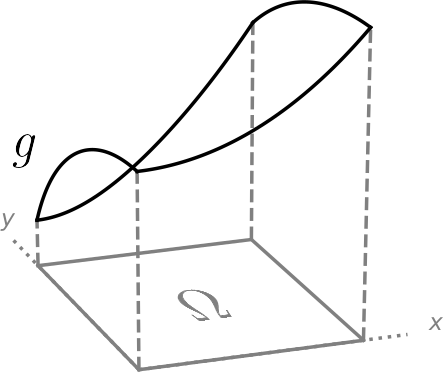
\includegraphics[width=1.15\textwidth]{images/omgcatenary.png}
\end{column}
\end{columns}
\end{frame}


\begin{frame}{minimal surfaces}

\centering
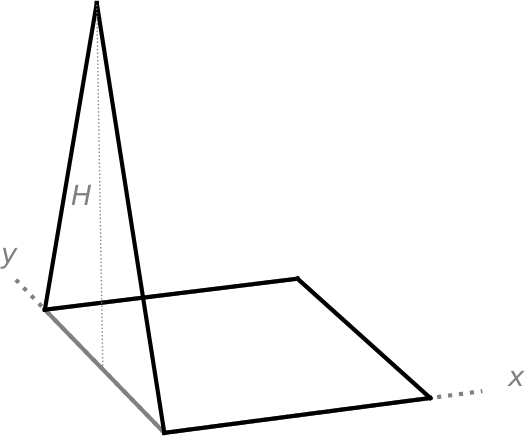
\includegraphics[width=0.3\textwidth]{images/tent.png} \qquad 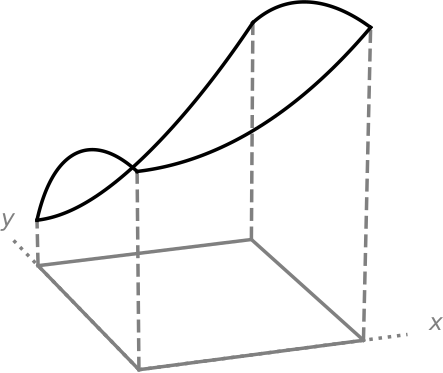
\includegraphics[width=0.3\textwidth]{images/catenary.png}

\mbox{{\scriptsize tent} \hspace{36mm} {\scriptsize catenoid}}

\bigskip
\begin{block}{minimal surface equation}
For given boundary function (wire frame) $g(x,y)$, find $u(x,y)$ so that
    $$-\Div \left(\frac{\grad u}{\sqrt{1 + |\grad u|^2}}\right) = 0 \quad \text{on } \Omega, \qquad u\big|_{\partial \Omega} = g.$$
\emph{Claim.}  In the absence of gravity, the surface $z=u(x,y)$ will be the shape of a soap bubble spanning $g$.
\end{block}
\end{frame}


\begin{frame}{a linear PDE problem}

\begin{columns}
\begin{column}{0.6\textwidth}
\begin{itemize}
\item I will consider only two PDEs today
    \begin{itemize}
    \item[1.] minimal surface equation \quad \emph{(nonlinear)}
    \item[2.] Poisson equation \quad \emph{(linear)}
    \end{itemize}
\item both are \alert{elliptic PDE boundary-value problems}
\item problem 2 is easier, so we will start there
\item note: $\Omega$ is a square in concrete examples
\end{itemize}
\end{column}
\begin{column}{0.4\textwidth}
\hfill 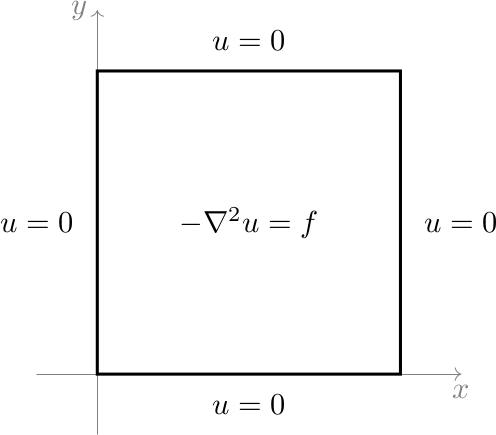
\includegraphics[width=\textwidth]{images/poisson.png}
\end{column}
\end{columns}

\bigskip
\begin{block}{\alert{Poisson equation} (with homogeneous boundary conditions)} For a given source function $f(x,y)$, find $u(x,y)$ so that
    $$-\grad^2 u = f \quad \text{on } \Omega, \qquad u\big|_{\partial \Omega} = 0.$$
\end{block}
\end{frame}


\begin{frame}{finite difference discretization}
\begin{columns}
\begin{column}{0.7\textwidth}
\begin{itemize}
\item PDEs are \alert{infinite-dimensional problems}
\item \alert{discretization} yields a finite system of equations in finitely-many unknowns
\item for example, via \alert{finite differences} (FD):
    $$f''(x) = \frac{f(x+h) - 2 f(x) + f(x-h)}{h^2} + O(h^2)$$
\item assume $\Omega = (0,1)^2$, and put a $m_x\times m_y$ grid on it
\item with spacings: \strut $h_x=\frac{1}{m_x-1}$, $h_y=\frac{1}{m_y-1}$
\item grid points: $(x_i,y_j) = (ih_x,jh_y)$ for $i=0,\dots,m_x-1$ and $j=0,\dots,m_y-1$
\item \alert{5-point stencil for the Laplacian}:
{\small
$$\grad^2 u(x_i,y_j) \approx \frac{u_{i-1,j} - 2 u_{ij} + u_{i+1,j}}{h_x^2} + \frac{u_{i,j-1} - 2 u_{ij} + u_{i,j+1}}{h_y^2}$$
}
\end{itemize}
\end{column}
\begin{column}{0.3\textwidth}
\hfill 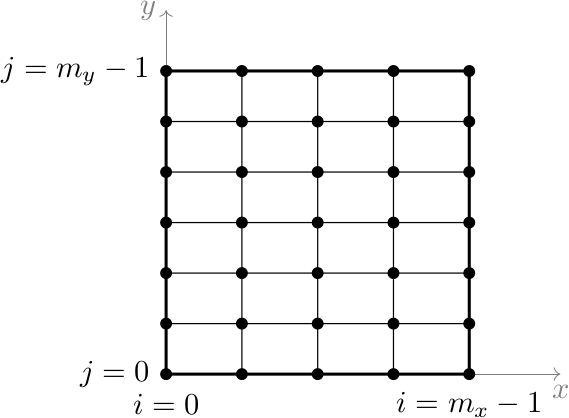
\includegraphics[width=\textwidth]{images/gridindexing.png}

\vspace{15mm}
\hfill 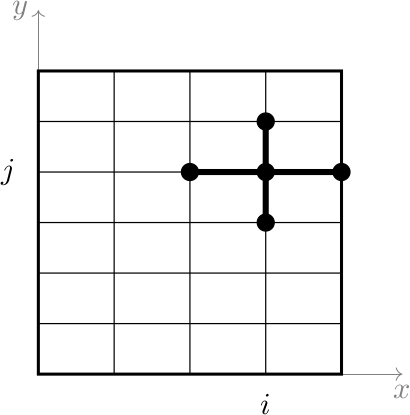
\includegraphics[width=0.7\textwidth]{images/gridstencil.png}
\end{column}
\end{columns}
\end{frame}


% next slide spy plots from Matlab (NOT OCTAVE):
%   m=5; spy(delsq(numgrid('S',m)),'k'), axis off,  print -dpdf lapspy5.pdf
%   m=8; spy(delsq(numgrid('S',m)),8,'k'), axis off,  print -dpdf lapspy8.pdf
% then pdfcrop

\begin{frame}{PDE \,$\stackrel{\text{discretize}}{\implies}$\, $A\,\bu=\bb$}
\begin{columns}
\begin{column}{0.73\textwidth}
\begin{itemize}
\item discretize $-\grad^2 u = f$ by FD:
	\begin{itemize}
	\item[$\circ$] $N=m_x m_y$ \, unknowns on the grid
	    \begin{itemize}
	    \item $m_x=4,m_y=3$ shown at right
        \end{itemize}
	\item[$\circ$] unknowns $\{u_{ij}\}$ are globally ordered: $u_\ell = u_{ij}$
	\end{itemize}
\item get a \alert{linear system for $\bu \in \RR^N$}:
	$$A\, \bu = \bb$$

	\begin{itemize}
	\item[$\circ$] $A \in \RR^{N\times N}$ is \alert{sparse}
	\item[$\circ$] $A$ is symmetric positive definite
	\item[$\circ$] $A$ has $O(1)$ nonzeros per row \hfill {\footnotesize \emph{$\leftarrow$ at most 5}}
	\item[$\circ$] $\bb \in \RR^N$ has entries $b_\ell = f(x_i,y_j)$
	\end{itemize}
\item examples at right:
	\begin{itemize}
	\item[$\circ$] for $m_x=m_y=5$: \quad \,\,\,9 non-trivial eqns
	\item[$\circ$] for $m_x=m_y=8$: \quad 36 non-trivial eqns
	\end{itemize}
\end{itemize}
\end{column}
\begin{column}{0.25\textwidth}
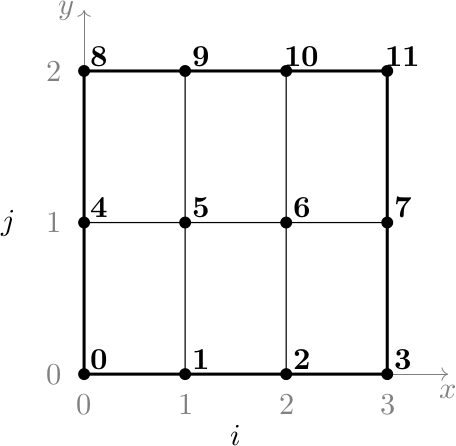
\includegraphics[width=\textwidth]{images/gridordering.png}

\medskip
\hfill 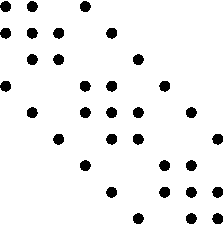
\includegraphics[width=0.7\textwidth]{images/lapspy5.pdf}

\smallskip
\hfill 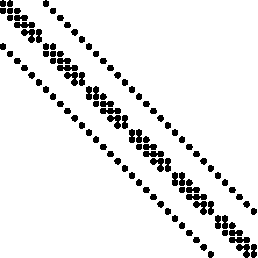
\includegraphics[width=0.7\textwidth]{images/lapspy8.pdf}
\end{column}
\end{columns}
\end{frame}


\begin{frame}{goal: solve $A\,\bu=\bb$ in $O(N)$ work}

\begin{itemize}
\item for our Poisson equation problem, the linear system
    $$A\,\bu=\bb$$
has $N$ unknowns
\item it can be set-up using $6N$ memory locations
	\begin{itemize}
	\item[$\circ$] $A$ has 5 nonzero entries per row, plus one entry of $\bb$
	\end{itemize}

\bigskip
\item can we solve $A\,\bu=\bb$ in $O(N)$ work and time as $N\to\infty$?
	\begin{itemize}
	\item[$\circ$] if so, the solver is \alert{optimal}
	\end{itemize}

\bigskip
\item let's back up and ask:

\medskip
\qquad what operations using our $A$ are obviously $O(N)$?
\end{itemize}
\end{frame}


\begin{frame}{cheap $O(N)$ operations: mat-vec and residual}

\begin{itemize}
\item we can compute $A\bv$ in $O(N)$ flops
	\begin{itemize}
	\item[$\circ$] this is because $A$ has $O(1)$ nonzero entries per row
	\item[$\circ$] and \alert{we do not need to do any work to multiply by zero}
	\end{itemize}

\bigskip
\begin{definition} given $\bv \in\RR^N$, the \alert{residual} for the linear system $A\,\bu=\bb$ is
	$$\br(\bv) = \bb - A\bv$$
observe that:
    $$A\,\bu = \bb \quad \iff \quad \br(\bu) = 0$$
\end{definition}

\item \alert{evaluating the residual is also an $O(N)$ operation}
\end{itemize}
\end{frame}


\section{simple iterations}

\begin{frame}{sometimes, simple iterations are cheap $O(N)$ operations}

\begin{definition} for the linear system $A\,\bu=\bb$ and an invertible matrix $M\in \RR^{N\times N}$, \alert{simple iteration} is
    $$\bv_{k+1} = \bv_k + \alpha\, M^{-1} \underbrace{\left(\bb - A \bv_k\right)}_{=\,\br(\bv_k)}$$
\end{definition}

\begin{itemize}
\item $\alpha\in\RR$ is a tuning parameter, with default $\alpha=1$
\item $M$ is called the \alert{preconditioner matrix} \dots next slide explains that
\item if $M=A$ and $\alpha=1$ then $\bv_{k+1}=\bu$, so one iteration solves it!
	\begin{itemize}
	\item[$\circ$] \dots not practical, and usually not $O(N)$
	\end{itemize}

\medskip
\item a simple iteration is $O(N)$ \dots \emph{if} $M$ is the right kind of matrix!
\end{itemize}
\end{frame}


\begin{frame}{preconditioned linear systems}

\begin{definition} if a matrix or linear map $M \in \RR^{N\times N}$ is invertible, we say
    $$M^{-1} A \bu = M^{-1} \bb$$
is a \alert{(left-) preconditioned} system for $A\,\bu=\bb$
\end{definition}

\begin{itemize}
\item the preconditioned system has the same solutions as before
\item the new residual is \, $\tilde{\br}(\bv) = M^{-1} (\bb - A \bv)$
\end{itemize}
\end{frame}


\begin{frame}{fast preconditioners?}

\begin{definition} a matrix or linear map $M$ is a \alert{fast preconditioner} if solving $M\,\bz=\bc$ requires $O(N)$ work
\end{definition}

\begin{itemize}
\item example: if $A$ has nonzero diagonal entries, the diagonal $M=D$ is a fast preconditioner
\item do \emph{not} actually form the matrix $M^{-1}$ when solving $M\,\bz=\bc$
\item warning: a preconditioner $M$ can be fast without being effective!
\item preconditioning is an apparently simple idea, but in 21st century it is used in all advanced solvers
\end{itemize}
\end{frame}


\begin{frame}{$O(N)$ simple iterations: Jacobi and Gauss-Seidel}
\begin{itemize}
\item split $A$ into diagonal and lower/upper triangular parts:
	$$A=D + L + U$$
\only<1>{
\item the linear system can be rearranged using the splitting:
\begin{align*}
A\,\bu=\bb \quad &\iff \quad D \bu = \bb - (L+U) \bu \\
               &\iff \quad \bu = \bu + D^{-1} (\bb - A \bu)
\end{align*}
\item solving $D\bz = \bc$ is $O(N)$
\begin{definition}
a \alert{Jacobi iteration} applies a fast preconditioner:
	$$\bv_{k+1} = \bv_k + D^{-1} (\bb - A \bv_k)$$
\end{definition}
}
\only<2>{
\item the linear system can be rearranged using the splitting:
\begin{align*}
A\,\bu=\bb \quad &\iff \quad (D+L) \bu = \bb - U \bu \\
               &\iff \quad \bu = \bu + (D+L)^{-1} (\bb - A \bu)
\end{align*}
\item solving $(D+L)\bz=\bc$ is $O(N)$ (for our $A$)

\begin{definition}
a \alert{Gauss-Seidel (GS) iteration} applies a fast preconditioner:
	$$\bv_{k+1} = \bv_k + (D+L)^{-1} (\bb - A \bv_k)$$
\end{definition}
}
\end{itemize}
\end{frame}


\begin{frame}{example of Gauss-Seidel iteration}
\begin{itemize}
\item matrix-splitting view obscures the simplicity of Gauss-Seidel
\item \emph{example}: consider the linear system $A\bu=\bb$ with
    $$A = \begin{bmatrix} 2 & -1 & & & & \\ -1 & 2 & -1 & & & \\ & -1 & 2 & -1 & & \\ & & \ddots & \ddots & \ddots & \\ & \Big. & & -1 & 2 & -1 \\ & & & & -1 & 2 \end{bmatrix}, \qquad \bb = \begin{bmatrix} b_1 \\ b_2 \\ b_3 \\ \vdots \\ b_N \end{bmatrix}$$

    \begin{itemize}
    \item[$\circ$] in this case, Gauss-Seidel iteration computes
    $$v_j^{[k+1]} = \frac{b_j}{2} + \frac{1}{2} \left(v_{j-1}^{[k+1]} + v_{j+1}^{[k]}\right)$$
    \item[$\circ$] this is a \alert{relaxation} method \dots update $v_j$ using average of neighbors
    \item[$\circ$] one can prove this method converges
    \item[$\circ$] this example is relevant because $A \sim -\grad^2$ in 1D
    \end{itemize}
\end{itemize}
\end{frame}


\begin{frame}{Jacobi and Gauss-Seidel iterations are bad \emph{as solvers}}

\begin{columns}
\begin{column}{0.5\textwidth}
\begin{itemize}
\item for Poisson problem linear system $A\bu=\bb$, one can prove Gauss- Seidel and Jacobi converge
\item but, after initial progress, residual norms decrease \alert{agonizingly slowly} on fine grids
\item an iteration $\bv_{k+1} = \phi(\bv_k)$ \emph{stagnates} or \emph{stalls} if the ratio of successive residual norms $\{\|\br(\bv_{k+1})\|/\|\br(\bv_k)\|\}$ goes to one
\end{itemize}
\end{column}
\begin{column}{0.5\textwidth}
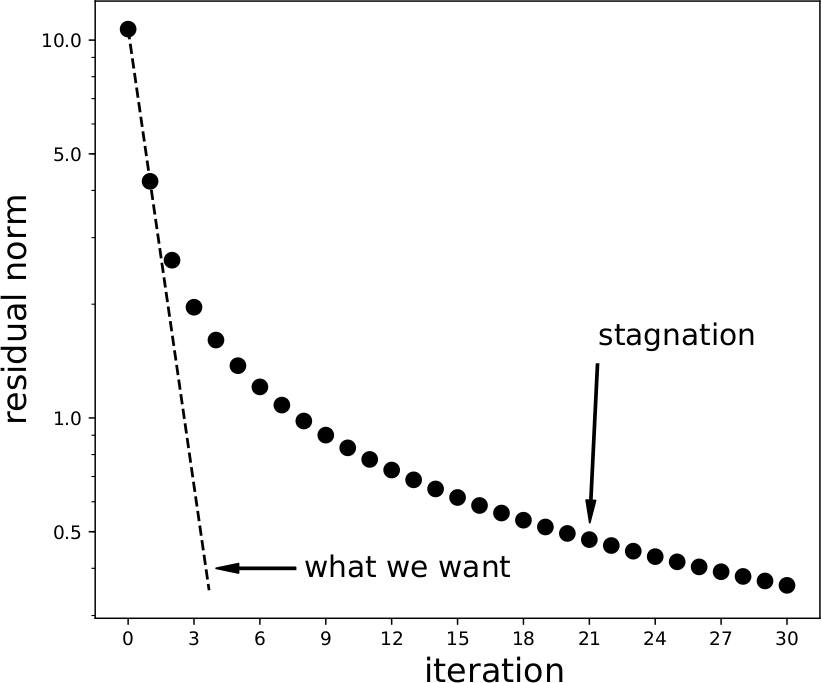
\includegraphics[width=\textwidth]{images/stagnation.png}
\end{column}
\end{columns}

\bigskip
\begin{itemize}
\item Achi Brandt, an inventor of multigrid:
\begin{quotation}
Stalling numerical processes must be wrong.  Whenever

the computer grinds very hard for small or slow effect,

there must be a better way to achieve the same goal.
\end{quotation}

\vspace{-16mm}
\hfill 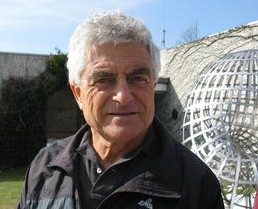
\includegraphics[width=0.1\textwidth]{images/abrandt.jpg}
\end{itemize}
\end{frame}


\begin{frame}{Jacobi and Gauss-Seidel iterations are good \emph{as smoothers}}
\begin{itemize}
\item observation: functions

become \emph{much smoother}

after a few iterations
\end{itemize}

\vspace{-15mm}

\only<1>{
\hfill 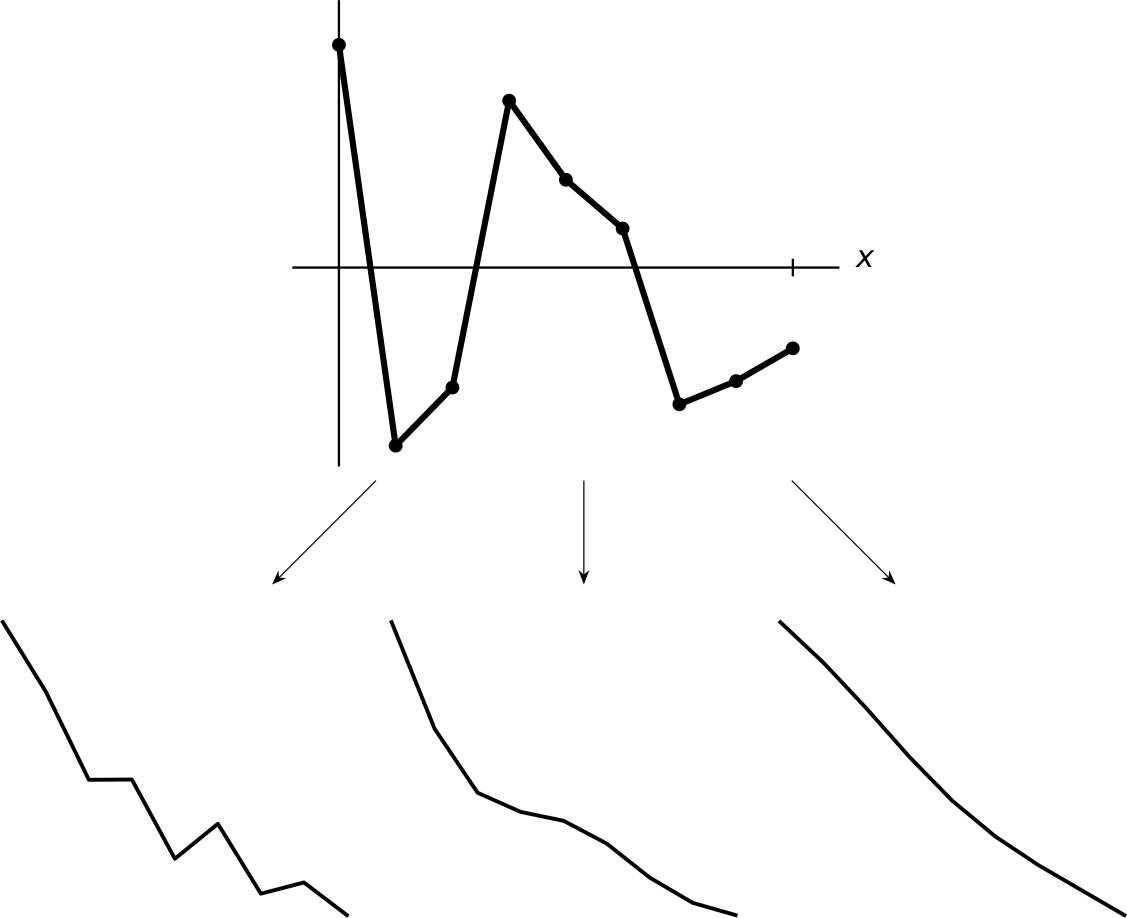
\includegraphics[height=0.8\textheight]{images/smoothing-space.png}
}
\only<2>{
\hfill 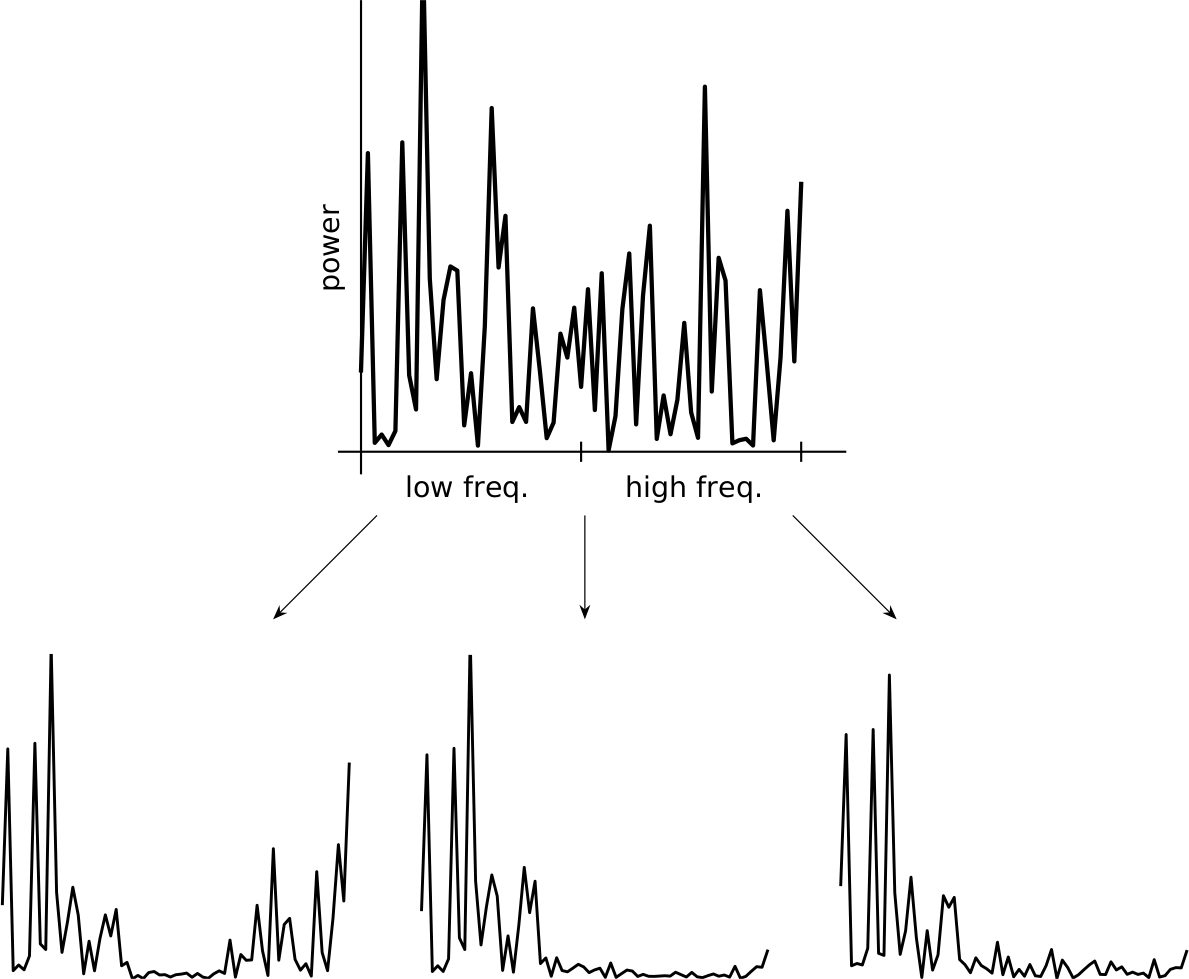
\includegraphics[height=0.8\textheight]{images/smoothing-freq.png}
}

\hfill {\scriptsize Jacobi \hspace{20mm} $\alpha=\frac{2}{3}$ Jacobi \hspace{14mm} Gauss-Seidel \hspace{6mm}}
\end{frame}


\section{2-grid method, and the coarse-grid correction}

\begin{frame}{grid transfers}

\begin{itemize}
\item multiple grid resolutions will allow us to exploit smoothers to generate fast solutions, but we need \alert{grid transfer} operators between the different grids

{\large
$$
\includegraphics[width=0.15\textwidth]{images/fine.png} \qquad
\begin{matrix}
\stackrel{\text{\texttt{restrict}}}{\longrightarrow} \\
\stackrel{\text{\texttt{prolong}}}{\longleftarrow} \\ \phantom{foo} \\ \phantom{foo}
\end{matrix}
\qquad 
\includegraphics[width=0.15\textwidth]{images/coarse.png}$$
}

\vspace{-8mm}
\item for a function $\bv$ defined on a finer grid, define its \alert{restriction} $R\bv$ to a coarser grid to be its value on the coarse grid points (\alert{injection}), or restrict by averaging onto the coarser grid (\emph{full weighting})
\item for a function $\bw$ defined on the coarser grid, define its \alert{prolongation} $P\bw$ to a finer grid by (linear) \emph{interpolation}
\item $R$, $P$ are linear operators
	\begin{itemize}
	\item[$\circ$] $R$, $P$ are rectangular (non-square) matrices
	\item[$\circ$] $R P = I$, or approximately so
	\end{itemize}
\end{itemize}
\end{frame}


\begin{frame}[fragile]
\frametitle{2-grid method}
\begin{itemize}
\item put these ideas together!
\item the \alert{2-grid method} approximately solves the PDE on the finer grid:

\bigskip
\begin{minted}[fontsize=\small,xleftmargin=10mm]{python}
def twogrid(v,pre=2,post=2):
    for k in range(pre):
         v = smooth(A,b,v)
    rc = restrict(b - A*v)
    ec = solve(Ac,rc)          # solve error equation
    v = v + prolong(ec)
    for k in range(post):
         v = smooth(A,b,v)
    return v
\end{minted}

\medskip
\item where
\begin{minted}[fontsize=\small,xleftmargin=10mm]{python}
A,b  = discretize(m,m)         # fine grid
Ac,_ = discretize(m/2,m/2)     # coarse grid
\end{minted}
\item \texttt{smooth()} does one Jacobi or GS iteration
\item \texttt{solve()} might be Gaussian elimination, etc., for \, $A^c \be^c = \br^c$
\end{itemize}
\end{frame}


\begin{frame}{the error equation}
\begin{itemize}
\item what do I mean by the ``error equation''?
\item for the linear system $A\,\bu=\bb$, consider some $\bv$ which is \emph{not} a solution

\begin{definition}
for any vector $\bv$, the \alert{error equation} corresponding to the linear system $A\,\bu = \bb$ is the equation
	$$A\,\be = \br(\bv)$$
\end{definition}

\item here's the logic:
\begin{align*}
    \be &= \bu - \bv                   &&\text{\emph{definition of the error}}\\
    A\, \be &= A \bu - A \bv           &&\text{\emph{multiply by $A$}}\\
    A\, \be &= \bb - A \bv = \br(\bv)  &&\text{\emph{error equation}}
\end{align*}
\end{itemize}
\end{frame}


\begin{frame}[fragile]
\frametitle{the coarse grid correction}
\begin{itemize}
\item the essential 3 lines in \,\texttt{twogrid()} form a \alert{coarse-grid correction}:

\medskip
\begin{minted}[fontsize=\small,xleftmargin=10mm]{python}
rc = restrict(b - A*v)     # restrict the residual
ec = solve(Ac,rc)          # coarse-grid solve
v = v + prolong(ec)        # add back as correction
\end{minted}

\smallskip
\item this is a kind of simple iteration: \qquad $\bv \leftarrow \bv + P (A^c)^{-1} R (\bb - A\bv)$
\item define the \emph{coarse-grid correction matrix}:
	$$B^c = P (A^c)^{-1} R$$
\item so \,\texttt{twogrid()} mixes two flavors of simple iteration:
\begin{align*}
\bv &\leftarrow \bv + M^{-1} (\bb - A\bv) &&\text{\emph{the smoother}} \\
\bv &\leftarrow \bv + B^c (\bb - A\bv) &&\text{\emph{the coarse-grid correction}}
\end{align*}

\medskip
\item Q: is $B^c \approx A^{-1}$?  \only<2>{\hspace{20mm} \alert{A: yes, but only for smooth inputs}}
\end{itemize}
\end{frame}


\begin{frame}[fragile]
\frametitle{2-grid method: the effect on error}
\begin{itemize}
\item look at \,\texttt{twogrid()} again:

\medskip
\begin{minted}[fontsize=\small,xleftmargin=10mm]{python}
def twogrid(v,pre=2,post=2):
    for k in range(pre):
         v = smooth(A,b,v)
    rc = restrict(b - A*v)
    ec = solve(Ac,rc)
    v = v + prolong(ec)
    for k in range(post):
         v = smooth(A,b,v)
    return v
\end{minted}

\bigskip
\item a fairly-quick calculation shows that \,\texttt{twogrid()} applies a linear operator, which is \alert{close to the zero operator}, to $\be=\bu-\bv$:
	$$\be \leftarrow (I - M^{-1} A)^{\text{\texttt{post}}} (I - B^c A) (I - M^{-1} A)^{\text{\texttt{pre}}} \be$$

\medskip
\item<2> Q: how should we solve the coarse-grid problem $A^c \be^c = \br^c$?
\end{itemize}
\end{frame}


\section{V-cycle multigrid}

\begin{frame}{hierarchy of grids}
\begin{itemize}
\item A: if we can have two levels of grids, we can have many!
\item when faced with a coarse-grid solve, just do another 2-grid \dots and keep going down to some really easy and cheap coarse grid

\bigskip\medskip
\hfill 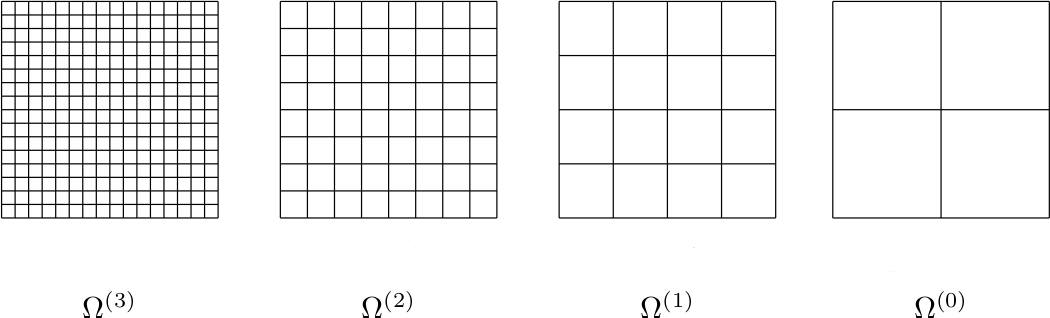
\includegraphics[width=0.8\textwidth]{images/multigrid-grids.png}

\medskip
\item restrictions $R$ and prolongations $P$ are needed in this \alert{grid hierarchy}

\end{itemize}
\end{frame}


\begin{frame}[fragile]
\frametitle{recursive V-cycle}
\begin{minted}[fontsize=\small,xleftmargin=10mm,texcomments]{python}
def vcycle(b,v,lev,pre=2,post=2):
    A,_ = discretize(lev)
    if lev == 0:
        return solve(A,b)    # the buck stops here
    for k in range(pre):
         v = smooth(A,b,v)
    rc = restrict(b - A*v)
    ec = vcycle(r,0,lev-1)   # descend a grid level
    v = v + prolong(ec)
    for k in range(post):
         v = smooth(A,b,v)
    return v
\end{minted}

\vspace{-5mm}
\hfill 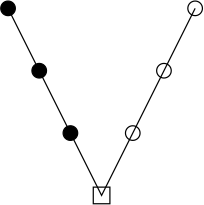
\includegraphics[width=0.15\textwidth]{images/vcycle.png}

\vspace{-8mm}
\hspace{5mm} 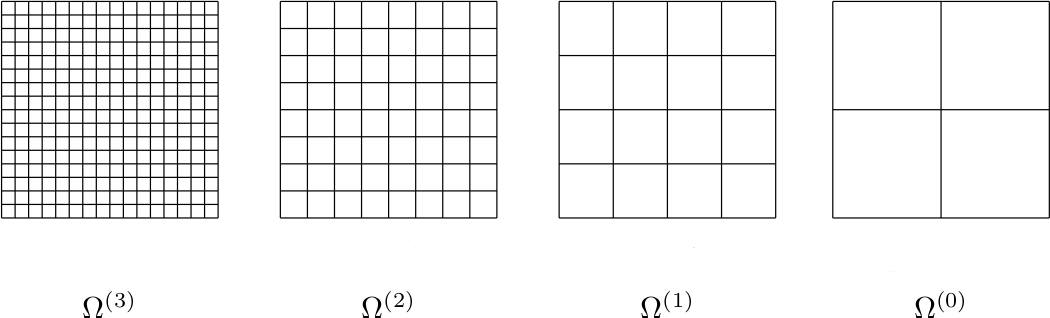
\includegraphics[width=0.6\textwidth]{images/multigrid-grids.png}
\end{frame}


\begin{frame}{how well does it work?}
\begin{itemize}
\item V-cycles work \alert{absurdly well} on the

Poisson problem \,$-\grad^2 u=f$

\vspace{-8mm}
\hfill 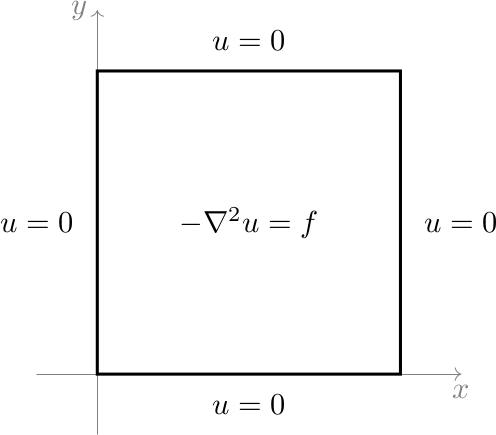
\includegraphics[width=0.3\textwidth]{images/poisson.png}

\vspace{-20mm}
\item scaling out to $m=4097$ ($N=1.6\times 10^7$):
\end{itemize}

\medskip
\begin{center}
\only<1>{ % Figure 7.2
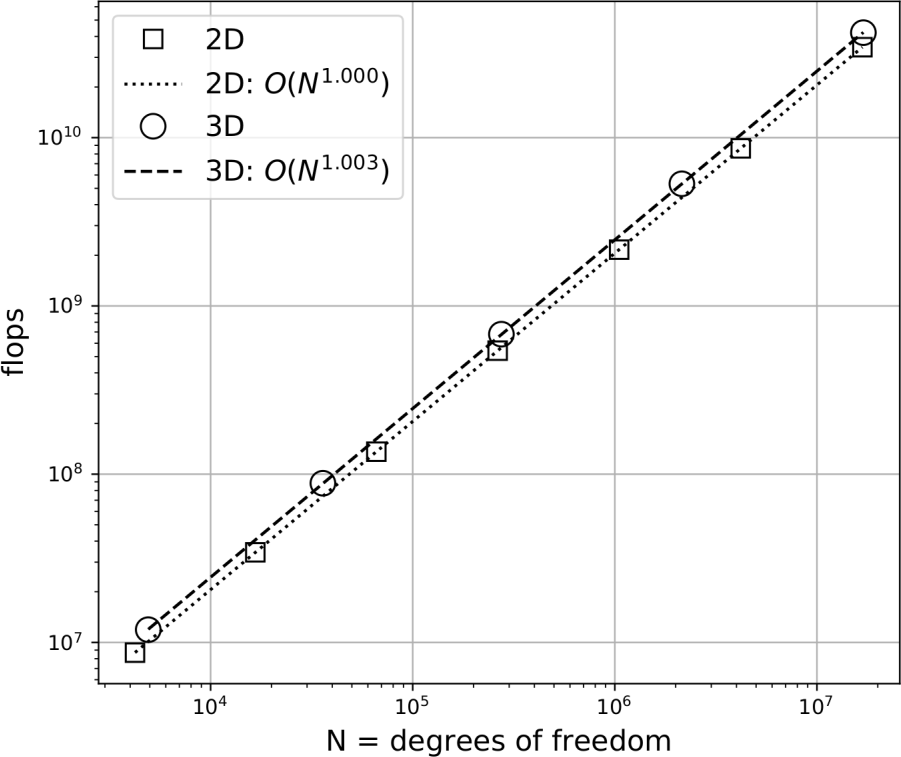
\includegraphics[height=0.54\textheight]{images/poisson-optimal-flops.png} \hspace{30mm}
}
\only<2>{ % Figure 7.4
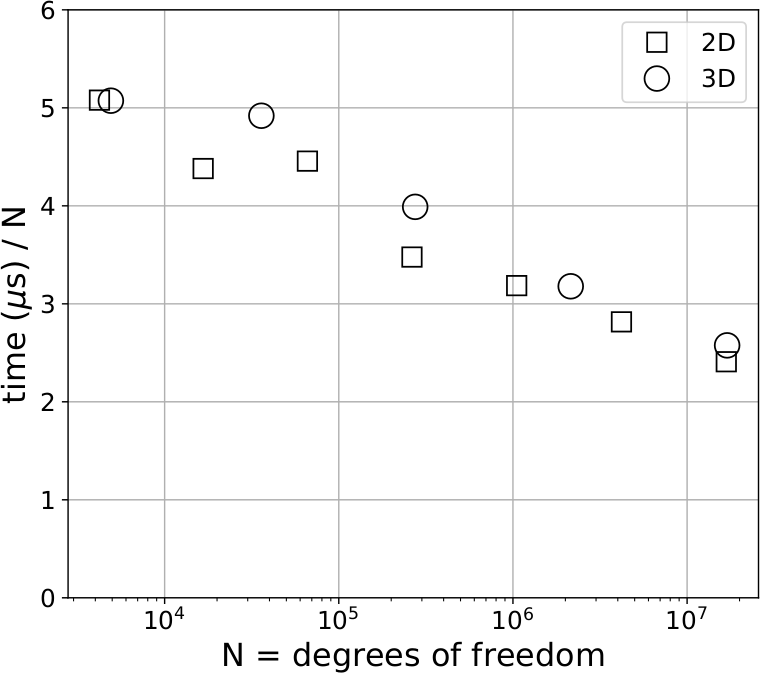
\includegraphics[height=0.54\textheight]{images/poisson-optimal-timeperdof.png} \hspace{30mm}
}
\end{center}
\end{frame}


\begin{frame}{on multigrid costs: single V-cycle}
\begin{itemize}
\item let us compute the work (flops) of applying a single V-cycle
    \begin{itemize}
    \item[$\circ$] note: multiple V-cycles are generally needed to solve the problem
    \end{itemize}

\medskip
\begin{definitions}

\vspace{-4mm}
\begin{align*}
|\Omega^{(k)}| &= (\text{number of grid points (unknowns) on grid $\Omega^{(k)}$}) \\
W_k^{k-1} &= \left(\begin{matrix} \text{smoother work done on grid $\Omega^{(k)}$, plus cost of} \\ \text{restriction/prolongation to/from next-coarser grid $\Omega^{(k-1)}$} \end{matrix}\right) \\
W_0 &= (\text{solver work done on the coarsest level})
\end{align*}
\end{definitions}

\medskip
\item $K=3$ case:
\end{itemize}

\vspace{-3mm}
\hfill 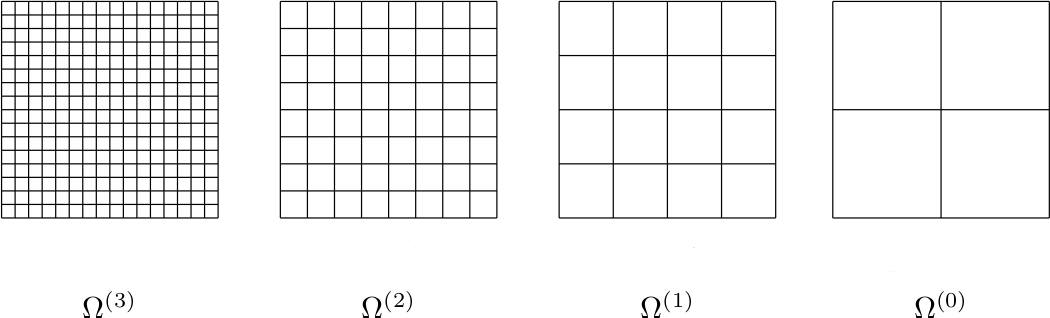
\includegraphics[width=0.65\textwidth]{images/multigrid-grids.png}
\end{frame}


\begin{frame}{on multigrid costs: single V-cycle}
\begin{itemize}
\item total cost of a single V-cycle:
    $$\overline{W} = W_K^{K-1} + W_{K-1}^{K-2} + \dots + W_1^0 + W_0$$
\item for 2D grids, each coarse grid is 4 times smaller:
    $$|\Omega^{(k-1)}| \approx \tfrac{1}{4} |\Omega^{(k)}|$$

\vspace{-28mm}
\hfill 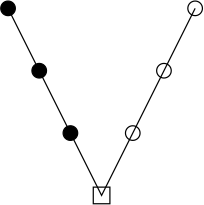
\includegraphics[width=0.13\textwidth]{images/vcycle.png}

\vspace{9mm}
\item since smoothers and restriction/prolongation are $O(1)$ per grid point:
    $$W_k^{k-1} \le C |\Omega^{(k)}|$$

    \begin{itemize}
    \item[$\circ$] for some $C$ independent of $k$
    \end{itemize}
\item<2> since $N=|\Omega^{(K)}|$ is the number of points in the finest grid,
\begin{align*}
\overline{W} &\le C |\Omega^{(K)}| + C |\Omega^{(K-1)}| + \dots + C |\Omega^{(1)}| + W_0 \\
    &\approx C N \left(1 + \tfrac{1}{4} + \dots + \tfrac{1}{4^{K-1}}\right) + W_0 \\
    &\approx C N \tfrac{1}{1-(1/4)} = \tfrac{4}{3} C N \hspace{20mm} \text{\alert{optimal}}
\end{align*}
\end{itemize}
\end{frame}


\begin{frame}{summary so far}
\begin{itemize}
\item multigrid combines 3 concepts:
\begin{enumerate}
\item classical iterations, such as Jacobi and GS, are \alert{cheap smoothers} of the residual and the error
\item a \alert{coarse-grid correction} does a good job of updating the fine-grid solution, if acting on a smooth residual
\item the coarse-grid correction is cheap because \alert{restriction and prolongation are cheap}
\end{enumerate}

\bigskip
\item but the Poisson problem is too easy!
\end{itemize}
\end{frame}


\section{nonlinear multigrid}

\begin{frame}{minimal surfaces, a nonlinear problem}

\centering
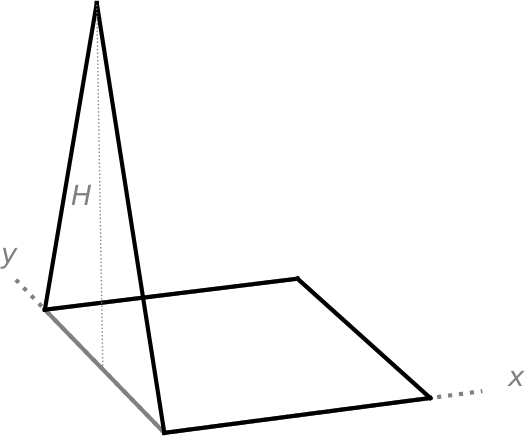
\includegraphics[width=0.3\textwidth]{images/tent.png} \qquad 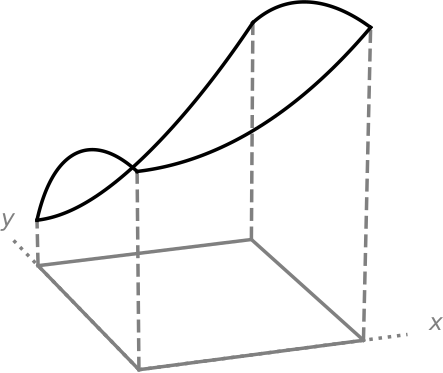
\includegraphics[width=0.3\textwidth]{images/catenary.png}

\mbox{{\scriptsize tent} \hspace{36mm} {\scriptsize catenoid}}

\bigskip
\begin{block}{minimal surface problem} for given boundary function (wire frame) $g(x,y)$, find $u(x,y)$ so that
    $$-\Div \left(\frac{\grad u}{\sqrt{1 + |\grad u|^2}}\right) = 0 \, \text{ on } \Omega, \qquad u\big|_{\partial \Omega} = g$$
\end{block}
\end{frame}


\begin{frame}{discretization gets you \dots more general equations}
\begin{itemize}
\item at each point $(x_i,y_j)$ on the target (finest) grid $\Omega^{(K)}$ we discretize to get an FD approximation of the PDE:
    $$f_{ij}(u_{i-1,j},\,u_{i+1,j},\,u_{i,j-1},\,u_{i,j+1},\,u_{i,j}) = 0$$

	\begin{itemize}
	\item[$\circ$] roughly-speaking, anyway ... see details next slide
	\item[$\circ$] unknowns must be globally-ordered into a vector $\bu \in \RR^N$:
	    $$u_\ell = u_{i,j}$$
    where $\ell=\ell(i,j)$ is a global-to-local indexing function
	\end{itemize}

\medskip
\begin{block}{nonlinear discretization principle}
enforcing the PDE at grid point $(x_i,y_j)$ gives one scalar equation $f_{ij}(\bu) = 0$
\end{block}

\bigskip
\item also globally-order the equations (functions), $f_\ell(\bu) = f_{ij}(\bu)$, to get a nonlinear system of $N$ scalar equations in $N$ scalar unknowns:
    $$\bF(\bu) = \bzero$$
\item $\bF$ is a sparse function, as each $f_\ell$ depends on only $O(1)$ entries of $\bu$
\end{itemize}
\end{frame}


\begin{frame}{details: 9-point stencil with staggered diffusivity}
\begin{itemize}
\item how do you discretize $\ds \Div \left(\frac{\grad u}{\sqrt{1 + |\grad u|^2}}\right)$?

\medskip
\item technique: generalize first!
\item discretize \,$\ds \Div \left(D(w) \grad u\right)$ where
\begin{align*}
D(w) &= (1+w)^{-1/2} \hspace{40mm} \\
w &= |\grad u|^2
\end{align*}

\vspace{-24mm}
\hfill 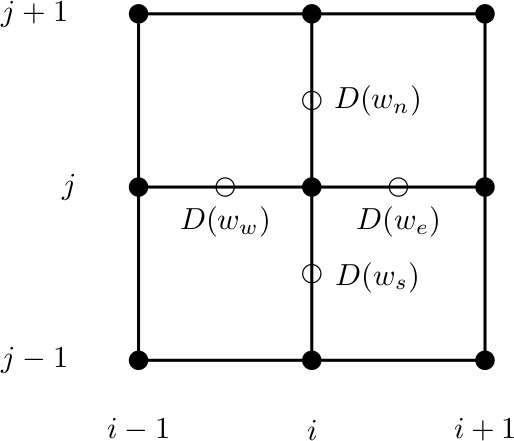
\includegraphics[width=0.3\textwidth]{images/msboxstencil.png}

\vspace{-8mm}
\item centered FD, using \emph{staggered} values of $D(w)$,

gets $O(h_x^2+h_y^2)$ truncation error and symmetry:

{\small
\begin{align*}
\Div \left(D(w) \grad u\right) &\approx \frac{D(w_e) (u_{i+1,j} - u_{i,j}) - D(w_w) (u_{i,j} - u_{i-1,j})}{h_x^2} \\
    &\qquad + \frac{D(w_n) (u_{i,j+1} - u_{i,j}) - D(w_s) (u_{i,j} - u_{i,j-1})}{h_y^2} \\
w_e = \left[|\grad u|^2\right]_{i+\frac{1}{2},j} &\approx \left(\frac{u_{i+1,j} - u_{i,j}}{h_x}\right)^2 + \left(\frac{u_{i,j+1} + u_{i+1,j+1} - u_{i,j} - u_{i+1,j}}{4 h_y}\right)^2 \hspace{10mm}
\end{align*}
}
\end{itemize}
\end{frame}


\begin{frame}{Newton's method \only<2>{and Jacobian management}}
\begin{itemize}
\item Q: how do we solve our nonlinear system $\bF(\bu)=\bzero$?

A: \alert{Newton's method}:
\begin{align*}
J(\bu^{p})\, \bs &= - \bF(\bu^p) \\
\bu^{p+1} &= \bu^p + \bs
\end{align*}
using the \alert{Jacobian matrix} \, $\displaystyle J(\bv)_{r,s} = \left[\,\frac{\partial f_r(\bv)}{\partial v_s}\,\right]$

\
\item<2> Q: how do you calculate the Jacobian?

\smallskip
A: compute derivatives on paper, and write code to evaluate it 

\smallskip
A: finite differencing again: \, $\displaystyle J(\bv)_{r,s} \approx \frac{f_r(\bv + \eps \bm{1}_s) - f_r(\bv)}{\eps}$

\smallskip
A: symbolically, and using powerful libraries
\end{itemize}
\end{frame}


\begin{frame}{details: 9-point stencil Jacobian sparsity}
\begin{itemize}
\item on a $6\times 6$ grid, the Jacobian $J(\bv)$ has this sparsity pattern:
\end{itemize}

\bigskip\bigskip
\begin{center}
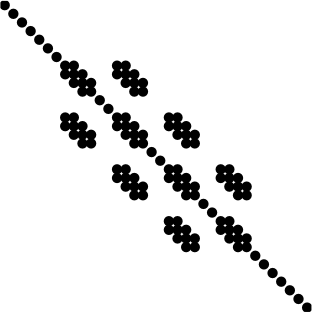
\includegraphics[width=0.4\textwidth]{images/minimal-spy.png}
\end{center}
\end{frame}


\begin{frame}[fragile]
\frametitle{Newton-multigrid}

\begin{itemize}
\item Q: how do you solve each linear system in the Newton iteration?

\medskip
A: solve \,$J(\bu^{p})\, \bs = - \bF(\bu^p)$ \,using \alert{multigrid}:

\medskip
\begin{minted}[fontsize=\small,xleftmargin=10mm,texcomments]{python}
def newtonmultigrid(v,cycles=1,levs):
    for p in ...:
         b = -F(v)
         s = 0
         for _ in range(cycles):
             s = vcycle(b,s,levs)
         v = v + s
    return v
\end{minted}
\end{itemize}
\end{frame}


\begin{frame}{nonlinear multigrid F-cycle solvers}
\begin{itemize}
\item Q: how do you find a good initial iterate $\bu^0$ for the Newton iteration?

\medskip
A: by solving the problem on a coarser grid, and prolonging

\medskip
\item this strategy is \alert{grid-sequencing}
    \begin{itemize}
    \item[$\circ$] justification: the domain of Newton convergence is larger on the smaller ($=$ coarser) version of the PDE
    \end{itemize}

\medskip
\item if you also solve at each level with Newton-multigrid, then this is a \alert{nonlinear F-cycle multigrid} \dots the most powerful solver!
\end{itemize}

\medskip
\begin{center}
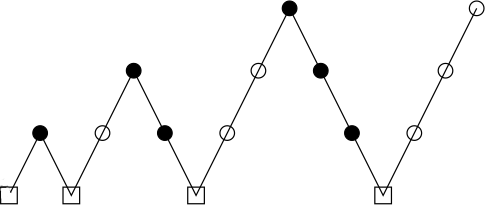
\includegraphics[width=0.5\textwidth]{images/multigrid-fullcycle.png}
\end{center}
\end{frame}


\begin{frame}[fragile]
\frametitle{minimal surface PDE problem: \textbf{live} demo}

\begin{itemize}
\item one open-source library which fully supports multigrid is \alert{PETSc}
    \begin{itemize}
    \item[$\circ$] PETSc $=$ portable, extensible toolkit for scientific computing \hfill \href{https://petsc.org/release/}{\texttt{petsc.org}}
    \item[$\circ$] it is inside the Python finite element library Firedrake \hfill {\scriptsize \href{https://www.firedrakeproject.org/index.html}{\texttt{firedrakeproject.org}}}
    \end{itemize}
\item this demo comes from Chapter 7 of my book \emph{PETSc for Partial Differential Equations} \hfill \href{https://github.com/bueler/p4pdes}{\texttt{github.com/bueler/p4pdes}}
\end{itemize}

\medskip
\begin{Verbatim}[fontsize=\footnotesize]
$ cd p4pdes/c/ch7/
$ make minimal

$ ./minimal -snes_fd_color -pc_type mg \
  -snes_grid_sequence 5 -snes_converged_reason

$ ./minimal -ms_problem tent -snes_fd_color -pc_type mg \
  -snes_grid_sequence 8 -snes_converged_reason \
  -snes_monitor_solution draw

$ mpiexec -n 6 ./minimal -ms_problem tent -snes_fd_color -pc_type mg \
  -snes_grid_sequence 9 -snes_converged_reason \
  -snes_view_solution vtk:u.vtr
$ paraview u.vtr
\end{Verbatim}
\end{frame}


\begin{frame}[fragile]
\frametitle{minimal surface PDE problem: the performance measurement}

\begin{itemize}
\item amount of arithmetic (flops) per degree of freedom (N)?
\item result: the \alert{solver is optimal} on this nonlinear minimal surface equation
    \begin{itemize}
    \item[$\circ$] but less so if the tent door is high
    \end{itemize}
\end{itemize}

\bigskip
\begin{center}
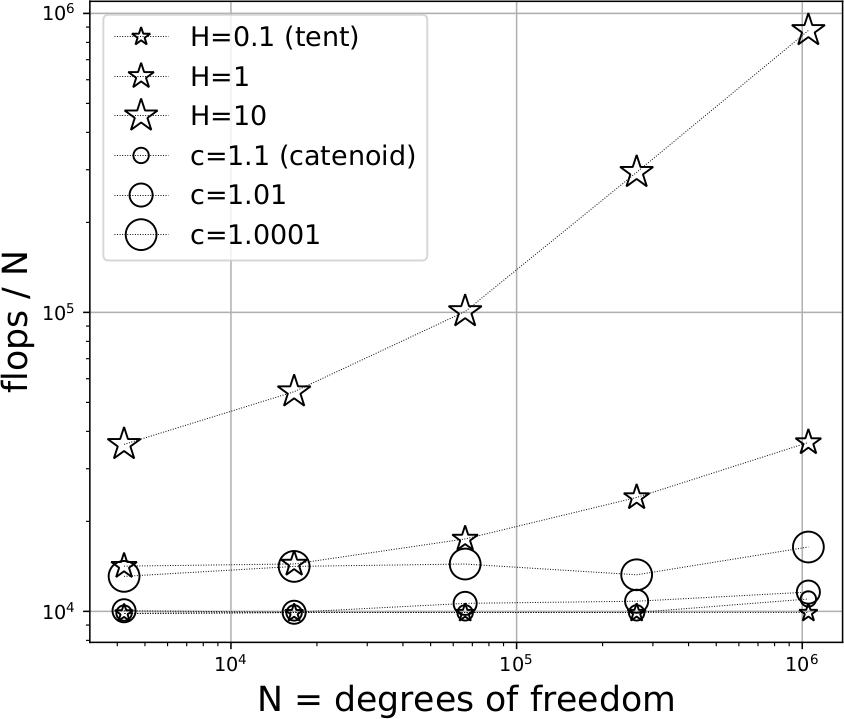
\includegraphics[width=0.5\textwidth]{images/minimal-flopsperdof.png}
\end{center}
\end{frame}


\begin{frame}{summary}
\begin{itemize}
\item a \alert{linear multigrid V-cycle} combines concepts to build an optimal solver for linear elliptic PDEs:
\begin{enumerate}
\item classical iterations are cheap smoothers
\item coarse-grid corrections act accurately on a smooth residual
\item restriction and prolongation are cheap
\end{enumerate}

\medskip
\item for nonlinear elliptic PDEs:
\begin{enumerate}
\item wrap a Newton iteration around multigrid V-cycles: \alert{Newton-multigrid}
\item add grid-sequencing to generate initial iterates on each finer grid
\item gives a \alert{nonlinear multigrid F-cycle solver}, optimal in many cases
\end{enumerate}

\medskip
\item other flavors of multigrid: \hfill {\color{gray}\small $\leftarrow$ different talks!}
    \begin{itemize}
    \item[$\circ$] full-approximation scheme (avoids the linearization in Newton's method)
    \item[$\circ$] linear algebraic multigrid (avoids hierarchy of grids)
    \end{itemize}
\end{itemize}
\end{frame}



\begin{frame}{references for learning about these ideas}

\setbeamerfont*{itemize/enumerate body}{size=\footnotesize}
\setbeamerfont*{itemize/enumerate subbody}{parent=itemize/enumerate body}

\begin{columns}
\begin{column}{0.8\textwidth}
\begin{itemize}
\item[] \textbf{A.~Brandt (1977)}. \emph{Multi-level adaptive solutions to boundary-value problems}, Mathematics of Computation 31 (138), 333--390
    \begin{itemize}
    \item[$\circ$] the origin of powerful multigrid, by its guru
    \end{itemize}

\medskip
\item[] \textbf{W.~Briggs, V.~E.~Henson, \& S.~McCormick (2000)}.  \emph{A Multigrid Tutorial}, 2nd ed., SIAM Press, Philadelphia
    \begin{itemize}
    \item[$\circ$] smaller, straightforward introduction
    \end{itemize}

\medskip
\item[] \textbf{E.~Bueler (2021)}. \emph{PETSc for Partial Differential Equations}, SIAM Press, Philadelphia
    \begin{itemize}
    \item[$\circ$] preconditioning ideas and diverse multigrid examples
    \item[$\circ$] for open-source C and Python codes, follow QR $\searrow$
    \end{itemize}

\medskip
\item[] \textbf{H.~Elman, D.~Silvester, \& A.~Wathen (2014)}. \emph{Finite Elements and Fast Iterative Solvers: With Applications to Incompressible Fluid Dynamics}, 2nd ed., Oxford U.~Press
    \begin{itemize}
    \item[$\circ$] multigrid in FE and fluids contexts
    \end{itemize}

\medskip
\item[] \textbf{U.~Trottenberg, C.~Oosterlee, \& A. Schuller (2001)}.  \emph{Multigrid}, Elsevier
    \begin{itemize}
    \item[$\circ$] comprehensive view, and theory
    \end{itemize}
\end{itemize}
\end{column}
\begin{column}{0.17\textwidth}
\hfill 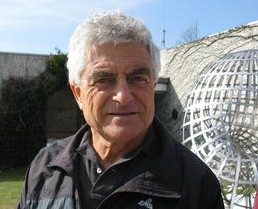
\includegraphics[width=0.7\textwidth]{images/abrandt.jpg}

\hfill {\scriptsize \emph{Achi Brandt}}

\vspace{7mm}
\hfill 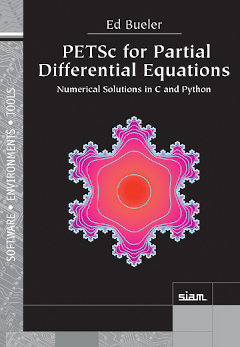
\includegraphics[width=0.9\textwidth]{images/bueler.jpg}

\medskip
\hfill 
\includegraphics[width=0.75\textwidth]{images/qrp4pdes.png}
\end{column}
\end{columns}
\end{frame}

\end{document}
